% SC1005 --- Chapter 5: Finite State Machines (0->100)
\chapter{Finite State Machines: Mealy, Moore, and Design}
\label{ch:fsm}

\begin{quote}
\emph{``A state machine is memory with a plan.''}
Combinational logic decides; sequential logic remembers; an FSM decides \emph{based on}
what it remembers. Every controller---from vending machine to CPU---is an FSM.
\end{quote}

\noindent\fbox{\parbox{\dimexpr\linewidth-2\fboxsep-2\fboxrule}{%
\textbf{From zero: states from scratch.} We define state, transition, and output,
then derive Mealy vs.\ Moore, state diagrams, and systematic synthesis from word problems.}}
\vspace{0.4em}

\section*{Learning Outcomes}
After this chapter you will be able to:
\begin{enumerate}[label=(L\arabic*)]
    \item define FSM state, transition function, and output function;
    \item distinguish Mealy and Moore machines and convert between them;
    \item draw state diagrams and tables from word-problem specifications;
    \item synthesise synchronous FSMs using D/JK flip-flops;
    \item minimise states via partition refinement and handle unused states.
\end{enumerate}

% ============================================================
\section{What Is a Finite State Machine?}
\label{sec:fsm-def}
An FSM is a 5-tuple $(S,I,O,\delta,\lambda)$: finite state set $S$, input alphabet $I$,
output alphabet $O$, next-state function $\delta:S\times I\to S$, output function $\lambda$.
On each clock edge, state advances $s^+=\delta(s,i)$ and output is produced.

Two output styles:
\begin{itemize}
    \item \textbf{Moore:} output depends on state only, $\lambda:S\to O$ (output changes only on clock edges---glitch-free but one cycle latency).
    \item \textbf{Mealy:} output depends on state \emph{and} input, $\lambda:S\times I\to O$ (faster response, but input glitches can propagate).
\end{itemize}

\begin{figure}[h]
\centering
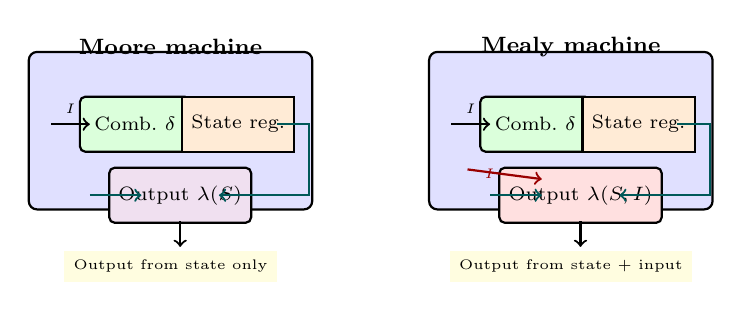
\begin{tikzpicture}[scale=0.82,every node/.style={font=\scriptsize}]
% Moore block
\node[draw,thick,fill=blue!12,minimum width=3.6cm,minimum height=2.0cm,rounded corners=3pt] (moore) at (2.0,0.45) {};
\node[font=\footnotesize\bfseries] at (2.0,1.75) {Moore machine};
\node[draw,thick,fill=green!14,minimum width=1.4cm,minimum height=0.7cm,rounded corners=2pt] at (1.45,0.55) {Comb.\ $\delta$};
\node[draw,thick,fill=orange!16,minimum width=1.05cm,minimum height=0.7cm] at (3.05,0.55) {State reg.};
\node[draw,thick,fill=violet!12,minimum width=1.15cm,minimum height=0.7cm,rounded corners=2pt] at (2.15,-0.55) {Output $\lambda(S)$};
\draw[->,thick] (0.15,0.55)--(0.75,0.55) node[midway,above,font=\tiny] {$I$};
\draw[->,thick,teal!70!black] (3.65,0.55)--(4.15,0.55)--(4.15,-0.55)--(2.75,-0.55);
\draw[->,thick,teal!70!black] (0.75,-0.55)--(1.55,-0.55);
\draw[->,thick] (2.15,-0.95)--(2.15,-1.35) node[below] {$O$};
\node[font=\tiny,fill=yellow!12] at (2.0,-1.65) {Output from state only};
% Mealy block
\begin{scope}[xshift=6.2cm]
\node[draw,thick,fill=blue!12,minimum width=3.6cm,minimum height=2.0cm,rounded corners=3pt] at (2.0,0.45) {};
\node[font=\footnotesize\bfseries] at (2.0,1.75) {Mealy machine};
\node[draw,thick,fill=green!14,minimum width=1.4cm,minimum height=0.7cm,rounded corners=2pt] at (1.45,0.55) {Comb.\ $\delta$};
\node[draw,thick,fill=orange!16,minimum width=1.05cm,minimum height=0.7cm] at (3.05,0.55) {State reg.};
\node[draw,thick,fill=red!12,minimum width=1.15cm,minimum height=0.7cm,rounded corners=2pt] at (2.15,-0.55) {Output $\lambda(S,I)$};
\draw[->,thick] (0.15,0.55)--(0.75,0.55) node[midway,above,font=\tiny] {$I$};
\draw[->,thick,teal!70!black] (3.65,0.55)--(4.15,0.55)--(4.15,-0.55)--(2.75,-0.55);
\draw[->,thick,teal!70!black] (0.75,-0.55)--(1.55,-0.55);
\draw[->,thick,red!60!black] (0.4,-0.15)--(1.55,-0.30) node[midway,left,font=\tiny] {$I$};
\draw[->,thick] (2.15,-0.95)--(2.15,-1.35) node[below] {$O$};
\node[font=\tiny,fill=yellow!12] at (2.0,-1.65) {Output from state + input};
\end{scope}
\end{tikzpicture}
\caption{Moore vs.\ Mealy: the only structural difference is whether input feeds the output logic (red arrow). State register is edge-triggered DFFs.}
\label{fig:moore-mealy}
\end{figure}

\section{State Diagrams and Tables}
\label{sec:state-diagram}
We specify FSMs by \emph{state diagrams} (circles = states, arcs = transitions labelled input/output)
or \emph{state tables} (rows = present state, columns = inputs). Example: sequence detector for $101$.

\begin{figure}[h]
\centering
\begin{tikzpicture}[scale=0.82,->,>=Stealth,auto,semithick,every node/.style={font=\scriptsize}]
% Moore sequence detector 101
\node[font=\footnotesize\bfseries] at (0,2.3) {Moore: detect $101$ (output $1$ in $S_3$)};
\node[state,fill=blue!12] (S0) at (0,0) {$S_0/0$};
\node[state,fill=green!14] (S1) at (3.0,0) {$S_1/0$};
\node[state,fill=orange!16] (S2) at (6.0,0) {$S_2/0$};
\node[state,fill=red!16] (S3) at (3.0,-1.85) {$S_3/1$};
\path (S0) edge[bend left=12] node {1} (S1)
      (S1) edge[bend left=12] node {0} (S2)
      (S2) edge[bend left=12] node {1} (S3)
      (S3) edge[bend left=10] node {0} (S2)
      (S0) edge[loop above] node {0} (S0)
      (S1) edge[loop above] node {1} (S1)
      (S2) edge[loop right] node {0} (S2)
      (S3) edge[loop below] node {1} (S1);
\node[font=\tiny,fill=yellow!12,rounded corners=1pt] at (3.0,-2.75) {Output is state label after `/'; glitch-free};
\end{tikzpicture}
\caption{Moore FSM that outputs $1$ when the last three inputs were $101$. State $S_i$ means ``last $i$ bits matched prefix of $101$''.}
\label{fig:seq-detector}
\end{figure}

The Mealy version needs only $3$ states (output on the arc $S_2 \xrightarrow{1/1} S_1$)
but its output can glitch if input glitches---tradeoff to choose per application.

\section{Synchronous Synthesis}
\label{sec:synthesis}
Five steps: (1) word problem $\to$ state diagram, (2) minimise states, (3) encode states in bits,
(4) derive next-state and output equations (K-maps), (5) implement with DFFs + combinational logic.

\begin{figure}[h]
\centering
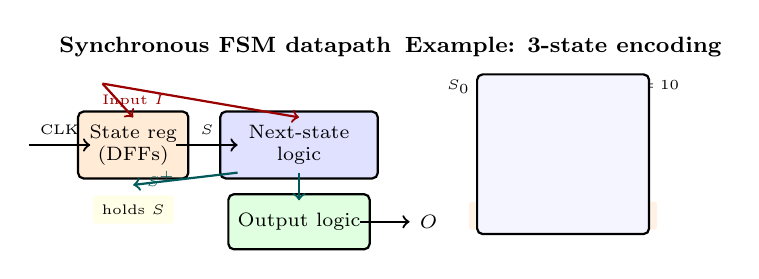
\begin{tikzpicture}[scale=0.78,every node/.style={font=\scriptsize}]
% Datapath: state reg + comb logic
\node[font=\footnotesize\bfseries] at (3.0,3.2) {Synchronous FSM datapath};
\node[draw,thick,fill=orange!16,minimum width=1.4cm,minimum height=0.85cm,rounded corners=2pt,align=center] (reg) at (1.5,1.6) {State reg\\(DFFs)};
\node[draw,thick,fill=blue!12,minimum width=2.0cm,minimum height=0.85cm,rounded corners=2pt,align=center] (next) at (4.2,1.6) {Next-state\\logic};
\node[draw,thick,fill=green!12,minimum width=1.65cm,minimum height=0.7cm,rounded corners=2pt] (out) at (4.2,0.35) {Output logic};
\draw[->,thick] (-0.2,1.6)--(0.8,1.6) node[midway,above,font=\tiny] {CLK};
\draw[->,thick] (2.2,1.6)--(3.2,1.6) node[midway,above,font=\tiny] {$S$};
\draw[->,thick,red!60!black] (1.0,2.6)--(1.5,2.05) node[above,font=\tiny] {Input $I$};
\draw[->,thick,red!60!black] (1.0,2.6)--(4.2,2.05);
\draw[->,thick,teal!70!black] (4.2,1.15)--(4.2,0.70);
\draw[->,thick] (5.2,0.35)--(6.0,0.35) node[right] {$O$};
\draw[->,thick,teal!70!black] (3.2,1.15)--(1.5,0.95) node[midway,left,font=\tiny] {$S^+$};
\node[font=\tiny,fill=yellow!10,rounded corners=1pt] at (1.5,0.55) {holds $S$};
% FSM example 3 states encoded 00 01 10
\begin{scope}[xshift=7.2cm]
\node[font=\footnotesize\bfseries] at (1.3,3.2) {Example: 3-state encoding};
\node[font=\tiny] at (1.3,2.55) {$S_0=00,\;S_1=01,\;S_2=10$};
\node[font=\tiny,align=left] at (1.3,1.85) {$D_1 = S_0\cdot I$};
\node[font=\tiny,align=left] at (1.3,1.45) {$D_0 = \bar S_1 S_0 + I$};
\node[font=\tiny,align=left] at (1.3,1.05) {$O = S_1$ (Moore)};
\node[font=\tiny,fill=orange!10,rounded corners=1pt] at (1.3,0.45) {unused $11\to00$ safe};
\draw[thick,rounded corners=2pt,fill=blue!4] (-0.1,2.75) rectangle (2.7,0.15);
\end{scope}
\end{tikzpicture}
\caption{Synchronous FSM hardware: state register holds present state; combinational blocks compute next state and output. Unused codes need safe next-state.}
\label{fig:fsm-datapath}
\end{figure}

\paragraph{State minimization.} Two states are equivalent if no input sequence distinguishes them
(same outputs and transitions to equivalent states). Iteratively partition states until stable---the
minimal machine is unique up to renaming (like DFA minimization).

\paragraph{Unused states.} With $k$ bits you get $2^k$ codes; if the FSM uses fewer, the remaining
codes are don't-cares for minimization but must transition to a safe state (often reset) to avoid lock-up.


\section{State Encoding and Mealy--Moore Interconversion}
Encoding choice affects cost and speed. \emph{Binary} uses $\lceil\log_2|S|\rceil$ bits (minimal flip-flops, more decoding).
\emph{One-hot} uses $|S|$ bits with one $1$ (more flip-flops, trivial next-state logic, fast, popular in FPGAs).
\emph{Gray} minimizes bit flips between adjacent states, reducing power and glitch risk in output-coded machines.

Mealy $\to$ Moore conversion: split each state by output value (Moore state = Mealy state + output memory), at most doubling states.
Moore $\to$ Mealy: keep states, move output from state label to incoming arcs---never needs more states.
\begin{example}[Traffic-light controller]
States GREEN, YELLOW, RED with timer inputs. Moore outputs drive lamps directly (glitch-free); Mealy would combine timer expiry and state
to anticipate the next lamp---one cycle faster but needs input synchronisation to avoid lamp flicker.
\end{example}

% ============================================================

% ============================================================
\section{Chapter Notes}
FSM theory originates with Mealy (1955) and Moore (1956), both at Bell Labs. Modern synthesis tools
extract FSMs from HDL case statements and optimise encoding (binary, one-hot, Gray) automatically.

% ============================================================
\section{ASM Charts and Algorithmic State Machines}
For larger controllers, state diagrams sprawl. An \emph{ASM (Algorithmic State Machine) chart} is a flowchart with three boxes:
state box (Moore outputs), decision diamond (input test), conditional output box (Mealy outputs). Each ASM block is one state + its
transitions, making translation to HDL (one \texttt{case} per state) mechanical.

ASM example: a simple CPU fetch--decode--execute controller has states FETCH, DECODE, EXECUTE with decision diamonds for
instruction opcode and conditional outputs for register enables and ALU op codes. Timing is still synchronous---every box
executes in one clock, diamond tests are combinational within the state.

% ============================================================

\paragraph{Mealy glitch vs.\ Moore latency.} Mealy output can change mid-cycle when input glitches, so any
asynchronous input must be synchronized before feeding Mealy output logic. Moore output is glitch-free between edges
but incurs one-cycle latency (input at cycle $k$ affects output at $k+1$). Many real controllers use Mealy internally
for speed and register the output (making it Moore at the pins)---best of both worlds.

\paragraph{Timing of FSM outputs.} In a synchronous FSM, next-state is computed combinationally from present state and inputs,
then clocked into DFFs. Output logic runs in parallel. Critical path $=t_{cq}+t_{next}+t_{su}$ (Moore) or
$t_{cq}+t_{next,out}+t_{su}$ (Mealy with input-to-output). Pipelining or one-hot encoding shortens $t_{next}$ at the cost of more flops.
Static timing analysis checks this path for every state transition.

\paragraph{State reduction example.} Two states with identical outputs and transitions to equivalent next states (under current partition)
merge without changing I/O behaviour. Repeatedly refine the partition until stable---the result is the minimal machine, unique up to renaming.
Lock-up states (no input leads to the valid cycle) must be broken by adding transitions to a safe reset state.

\section{Exercises}
\label{sec:ch05-exercises}
\begin{enumerate}[label=E5.\arabic*, leftmargin=*, itemsep=0.8em]
    \item \textbf{Mealy vs.\ Moore.} Convert the Moore $101$ detector in Fig.~\ref{fig:seq-detector} to Mealy. How many states? Compare output timing on a timing diagram.
    \item \textbf{Vending machine.} Design a Moore FSM for a vending machine: inputs nickel/dime, product costs 15\textcent, output `dispense'. Draw diagram and state table.
    \item \textbf{Synthesis.} Synthesise the 3-state FSM in Fig.~\ref{fig:fsm-datapath} using D flip-flops. Write K-maps for $D_1,D_0$ and draw the gate-level circuit.
    \item \textbf{Minimization.} A FSM has 6 states with given table (provide). Apply partition refinement to find the minimal equivalent machine. Is it unique?
    \item \textbf{One-hot vs.\ binary.} Encode a 4-state FSM in binary (2 bits) and one-hot (4 bits). Compare flip-flop count, next-state logic complexity, and speed.
\end{enumerate}
% End of Chapter 5
